\documentclass[12pt,a4paper]{article}

\usepackage[a4paper,text={16.5cm,25.2cm},centering]{geometry}
\usepackage{lmodern}
\usepackage{amssymb,amsmath}
\usepackage{bm}
\usepackage{graphicx}
\usepackage{microtype}
\usepackage{hyperref}
\setlength{\parindent}{0pt}
\setlength{\parskip}{1.2ex}

\hypersetup
       {   pdfauthor = { Sheehan Olver },
           pdftitle={ foo },
           colorlinks=TRUE,
           linkcolor=black,
           citecolor=blue,
           urlcolor=blue
       }




\usepackage{upquote}
\usepackage{listings}
\usepackage{xcolor}
\lstset{
    basicstyle=\ttfamily\footnotesize,
    upquote=true,
    breaklines=true,
    breakindent=0pt,
    keepspaces=true,
    showspaces=false,
    columns=fullflexible,
    showtabs=false,
    showstringspaces=false,
    escapeinside={(*@}{@*)},
    extendedchars=true,
}
\newcommand{\HLJLt}[1]{#1}
\newcommand{\HLJLw}[1]{#1}
\newcommand{\HLJLe}[1]{#1}
\newcommand{\HLJLeB}[1]{#1}
\newcommand{\HLJLo}[1]{#1}
\newcommand{\HLJLk}[1]{\textcolor[RGB]{148,91,176}{\textbf{#1}}}
\newcommand{\HLJLkc}[1]{\textcolor[RGB]{59,151,46}{\textit{#1}}}
\newcommand{\HLJLkd}[1]{\textcolor[RGB]{214,102,97}{\textit{#1}}}
\newcommand{\HLJLkn}[1]{\textcolor[RGB]{148,91,176}{\textbf{#1}}}
\newcommand{\HLJLkp}[1]{\textcolor[RGB]{148,91,176}{\textbf{#1}}}
\newcommand{\HLJLkr}[1]{\textcolor[RGB]{148,91,176}{\textbf{#1}}}
\newcommand{\HLJLkt}[1]{\textcolor[RGB]{148,91,176}{\textbf{#1}}}
\newcommand{\HLJLn}[1]{#1}
\newcommand{\HLJLna}[1]{#1}
\newcommand{\HLJLnb}[1]{#1}
\newcommand{\HLJLnbp}[1]{#1}
\newcommand{\HLJLnc}[1]{#1}
\newcommand{\HLJLncB}[1]{#1}
\newcommand{\HLJLnd}[1]{\textcolor[RGB]{214,102,97}{#1}}
\newcommand{\HLJLne}[1]{#1}
\newcommand{\HLJLneB}[1]{#1}
\newcommand{\HLJLnf}[1]{\textcolor[RGB]{66,102,213}{#1}}
\newcommand{\HLJLnfm}[1]{\textcolor[RGB]{66,102,213}{#1}}
\newcommand{\HLJLnp}[1]{#1}
\newcommand{\HLJLnl}[1]{#1}
\newcommand{\HLJLnn}[1]{#1}
\newcommand{\HLJLno}[1]{#1}
\newcommand{\HLJLnt}[1]{#1}
\newcommand{\HLJLnv}[1]{#1}
\newcommand{\HLJLnvc}[1]{#1}
\newcommand{\HLJLnvg}[1]{#1}
\newcommand{\HLJLnvi}[1]{#1}
\newcommand{\HLJLnvm}[1]{#1}
\newcommand{\HLJLl}[1]{#1}
\newcommand{\HLJLld}[1]{\textcolor[RGB]{148,91,176}{\textit{#1}}}
\newcommand{\HLJLs}[1]{\textcolor[RGB]{201,61,57}{#1}}
\newcommand{\HLJLsa}[1]{\textcolor[RGB]{201,61,57}{#1}}
\newcommand{\HLJLsb}[1]{\textcolor[RGB]{201,61,57}{#1}}
\newcommand{\HLJLsc}[1]{\textcolor[RGB]{201,61,57}{#1}}
\newcommand{\HLJLsd}[1]{\textcolor[RGB]{201,61,57}{#1}}
\newcommand{\HLJLsdB}[1]{\textcolor[RGB]{201,61,57}{#1}}
\newcommand{\HLJLsdC}[1]{\textcolor[RGB]{201,61,57}{#1}}
\newcommand{\HLJLse}[1]{\textcolor[RGB]{59,151,46}{#1}}
\newcommand{\HLJLsh}[1]{\textcolor[RGB]{201,61,57}{#1}}
\newcommand{\HLJLsi}[1]{#1}
\newcommand{\HLJLso}[1]{\textcolor[RGB]{201,61,57}{#1}}
\newcommand{\HLJLsr}[1]{\textcolor[RGB]{201,61,57}{#1}}
\newcommand{\HLJLss}[1]{\textcolor[RGB]{201,61,57}{#1}}
\newcommand{\HLJLssB}[1]{\textcolor[RGB]{201,61,57}{#1}}
\newcommand{\HLJLnB}[1]{\textcolor[RGB]{59,151,46}{#1}}
\newcommand{\HLJLnbB}[1]{\textcolor[RGB]{59,151,46}{#1}}
\newcommand{\HLJLnfB}[1]{\textcolor[RGB]{59,151,46}{#1}}
\newcommand{\HLJLnh}[1]{\textcolor[RGB]{59,151,46}{#1}}
\newcommand{\HLJLni}[1]{\textcolor[RGB]{59,151,46}{#1}}
\newcommand{\HLJLnil}[1]{\textcolor[RGB]{59,151,46}{#1}}
\newcommand{\HLJLnoB}[1]{\textcolor[RGB]{59,151,46}{#1}}
\newcommand{\HLJLoB}[1]{\textcolor[RGB]{102,102,102}{\textbf{#1}}}
\newcommand{\HLJLow}[1]{\textcolor[RGB]{102,102,102}{\textbf{#1}}}
\newcommand{\HLJLp}[1]{#1}
\newcommand{\HLJLc}[1]{\textcolor[RGB]{153,153,119}{\textit{#1}}}
\newcommand{\HLJLch}[1]{\textcolor[RGB]{153,153,119}{\textit{#1}}}
\newcommand{\HLJLcm}[1]{\textcolor[RGB]{153,153,119}{\textit{#1}}}
\newcommand{\HLJLcp}[1]{\textcolor[RGB]{153,153,119}{\textit{#1}}}
\newcommand{\HLJLcpB}[1]{\textcolor[RGB]{153,153,119}{\textit{#1}}}
\newcommand{\HLJLcs}[1]{\textcolor[RGB]{153,153,119}{\textit{#1}}}
\newcommand{\HLJLcsB}[1]{\textcolor[RGB]{153,153,119}{\textit{#1}}}
\newcommand{\HLJLg}[1]{#1}
\newcommand{\HLJLgd}[1]{#1}
\newcommand{\HLJLge}[1]{#1}
\newcommand{\HLJLgeB}[1]{#1}
\newcommand{\HLJLgh}[1]{#1}
\newcommand{\HLJLgi}[1]{#1}
\newcommand{\HLJLgo}[1]{#1}
\newcommand{\HLJLgp}[1]{#1}
\newcommand{\HLJLgs}[1]{#1}
\newcommand{\HLJLgsB}[1]{#1}
\newcommand{\HLJLgt}[1]{#1}



\def\qqand{\qquad\hbox{and}\qquad}
\def\qqfor{\qquad\hbox{for}\qquad}
\def\qqas{\qquad\hbox{as}\qquad}
\def\D{ {\rm d} }
\def\I{ {\rm i} }
\def\E{ {\rm e} }
\def\C{ {\mathbb C} }
\def\R{ {\mathbb R} }
\def\CC{ {\cal C} }
\def\HH{ {\cal H} }
\def\LL{ {\cal L} }
\def\vc#1{ {\mathbf #1} }
\def\bbC{ {\mathbb C} }

\def\qqqquad{\qquad\qquad}
\def\qqwhere{\qquad\hbox{where}\qquad}
\def\Res_#1{\underset{#1}{\rm Res}\,}
\def\sech{ {\rm sech}\, }
\def\acos{ {\rm acos}\, }
\def\atan{ {\rm atan}\, }
\def\upepsilon{\varepsilon}


\def\Xint#1{ \mathchoice
   {\XXint\displaystyle\textstyle{#1} }%
   {\XXint\textstyle\scriptstyle{#1} }%
   {\XXint\scriptstyle\scriptscriptstyle{#1} }%
   {\XXint\scriptscriptstyle\scriptscriptstyle{#1} }%
   \!\int}
\def\XXint#1#2#3{ {\setbox0=\hbox{$#1{#2#3}{\int}$}
     \vcenter{\hbox{$#2#3$}}\kern-.5\wd0} }
\def\ddashint{\Xint=}
\def\dashint{\Xint-}
% \def\dashint
\def\infdashint{\dashint_{-\infty}^\infty}




\def\addtab#1={#1\;&=}
\def\ccr{\\\addtab}
\def\ip<#1>{\left\langle{#1}\right\rangle}
\def\dx{\D x}
\def\dt{\D t}
\def\dz{\D z}

\def\norm#1{\left\| #1 \right\|}

\def\pr(#1){\left({#1}\right)}
\def\br[#1]{\left[{#1}\right]}

\def\abs#1{\left|{#1}\right|}
\def\fpr(#1){\!\pr({#1})}

\def\sopmatrix#1{ \begin{pmatrix}#1\end{pmatrix} }

\def\endash{–}
\def\mdblksquare{\blacksquare}
\def\lgblksquare{\blacksquare}
\def\scre{\E}
\def\mapengine#1,#2.{\mapfunction{#1}\ifx\void#2\else\mapengine #2.\fi }

\def\map[#1]{\mapengine #1,\void.}

\def\mapenginesep_#1#2,#3.{\mapfunction{#2}\ifx\void#3\else#1\mapengine #3.\fi }

\def\mapsep_#1[#2]{\mapenginesep_{#1}#2,\void.}


\def\vcbr[#1]{\pr(#1)}


\def\bvect[#1,#2]{
{
\def\dots{\cdots}
\def\mapfunction##1{\ | \  ##1}
	\sopmatrix{
		 \,#1\map[#2]\,
	}
}
}



\def\vect[#1]{
{\def\dots{\ldots}
	\vcbr[{#1}]
} }

\def\vectt[#1]{
{\def\dots{\ldots}
	\vect[{#1}]^{\top}
} }

\def\Vectt[#1]{
{
\def\mapfunction##1{##1 \cr} 
\def\dots{\vdots}
	\begin{pmatrix}
		\map[#1]
	\end{pmatrix}
} }

\def\addtab#1={#1\;&=}
\def\ccr{\\\addtab}

\begin{document}

\textbf{M3M6: Applied Complex Analysis}

Dr. Sheehan Olver

s.olver@imperial.ac.uk

\section{Lecture 11: Representing analytic functions by their behaviour near singularities}
A \emph{key} theme in complex analysis is representing functions by their behaviour near singularities.   A simple example of this is partial fraction expansion: a rational function $p(z)/q(z)$ can be expressed as a sum of its behaviour near poles and infinity. This is more complicated, but doable in a systematic manner for functions with branch cuts.  In this lecture we:

\begin{itemize}
\item[1. ] Derive partial fraction expansion using Cauchy's integral formula


\item[2. ] Recoverying functions like $\sqrt(z-1)\sqrt(z+1)$ from their behaviour on the branch cut

\end{itemize}
\subsection{Partial fraction expansion}
\textbf{Corollary (Cauchy's integral representation around holes)} Let $D \subset {\mathbb C}$ be a domain with $g$ holes (i.e., genus $g$).  Suppose $f$ is holmorphic in and on the boundary of $D$.  Given $g$ simple closed negatively oriented contours   surrounding the holes $\gamma_1, \ldots, \gamma_g$ and a simple closed positively oriented contour $\gamma_\infty$ surrounding   the outer boundary of $D$, we have

\[
f(z) = {1 \over 2 \pi \I} \br[\sum_{k=1}^{g} \oint_{\gamma_k} + \oint_{\gamma_\infty}] {f(\zeta) \over \zeta - z} \D \zeta
\]
Here are is an example. Consider 

\[
f(z) = (\E^{1/z} + \E^z) / (z (z+2))
\]
which has an essential singularity at 0 and $\infty$ and a simple pole at $2$.  We can recover $f$ from contours around each singularity:


\begin{lstlisting}
(*@\HLJLk{using}@*) (*@\HLJLn{ApproxFun}@*)(*@\HLJLp{,}@*) (*@\HLJLn{ComplexPhasePortrait}@*)(*@\HLJLp{,}@*) (*@\HLJLn{Plots}@*)
(*@\HLJLn{f}@*) (*@\HLJLoB{=}@*) (*@\HLJLn{z}@*) (*@\HLJLoB{->}@*) (*@\HLJLp{(}@*)(*@\HLJLnf{exp}@*)(*@\HLJLp{(}@*)(*@\HLJLni{1}@*)(*@\HLJLoB{/}@*)(*@\HLJLn{z}@*)(*@\HLJLp{)}@*) (*@\HLJLoB{+}@*) (*@\HLJLnf{exp}@*)(*@\HLJLp{(}@*)(*@\HLJLn{z}@*)(*@\HLJLp{))}@*)(*@\HLJLoB{/}@*)(*@\HLJLp{(}@*)(*@\HLJLn{z}@*)(*@\HLJLoB{*}@*)(*@\HLJLp{(}@*)(*@\HLJLn{z}@*)(*@\HLJLoB{+}@*)(*@\HLJLni{2}@*)(*@\HLJLp{))}@*)
(*@\HLJLn{\ensuremath{\Gamma}}@*) (*@\HLJLoB{=}@*) (*@\HLJLnf{Circle}@*)(*@\HLJLp{(}@*)(*@\HLJLnfB{0.0}@*)(*@\HLJLp{,}@*) (*@\HLJLnfB{4.0}@*)(*@\HLJLp{)}@*) (*@\HLJLoB{\ensuremath{\cup}}@*) (*@\HLJLnf{Circle}@*)(*@\HLJLp{(}@*)(*@\HLJLnfB{0.0}@*)(*@\HLJLp{,}@*)(*@\HLJLnfB{0.5}@*)(*@\HLJLp{,}@*)(*@\HLJLkc{false}@*)(*@\HLJLp{)}@*) (*@\HLJLoB{\ensuremath{\cup}}@*) (*@\HLJLnf{Circle}@*)(*@\HLJLp{(}@*)(*@\HLJLoB{-}@*)(*@\HLJLnfB{2.0}@*)(*@\HLJLp{,}@*)(*@\HLJLnfB{0.1}@*)(*@\HLJLp{,}@*)(*@\HLJLkc{false}@*)(*@\HLJLp{)}@*)
(*@\HLJLnf{phaseplot}@*)(*@\HLJLp{(}@*)(*@\HLJLoB{-}@*)(*@\HLJLnfB{5..5}@*)(*@\HLJLp{,}@*) (*@\HLJLoB{-}@*)(*@\HLJLnfB{5..5}@*)(*@\HLJLp{,}@*) (*@\HLJLn{f}@*)(*@\HLJLp{)}@*)
(*@\HLJLnf{plot!}@*)(*@\HLJLp{(}@*)(*@\HLJLn{\ensuremath{\Gamma}}@*)(*@\HLJLp{;}@*) (*@\HLJLn{color}@*)(*@\HLJLoB{=:}@*)(*@\HLJLn{black}@*)(*@\HLJLp{,}@*) (*@\HLJLn{label}@*)(*@\HLJLoB{=:}@*)(*@\HLJLn{contour}@*)(*@\HLJLp{,}@*) (*@\HLJLn{arrow}@*)(*@\HLJLoB{=}@*)(*@\HLJLkc{true}@*)(*@\HLJLp{,}@*) (*@\HLJLn{linewidth}@*)(*@\HLJLoB{=}@*)(*@\HLJLnfB{1.5}@*)(*@\HLJLp{)}@*)
\end{lstlisting}

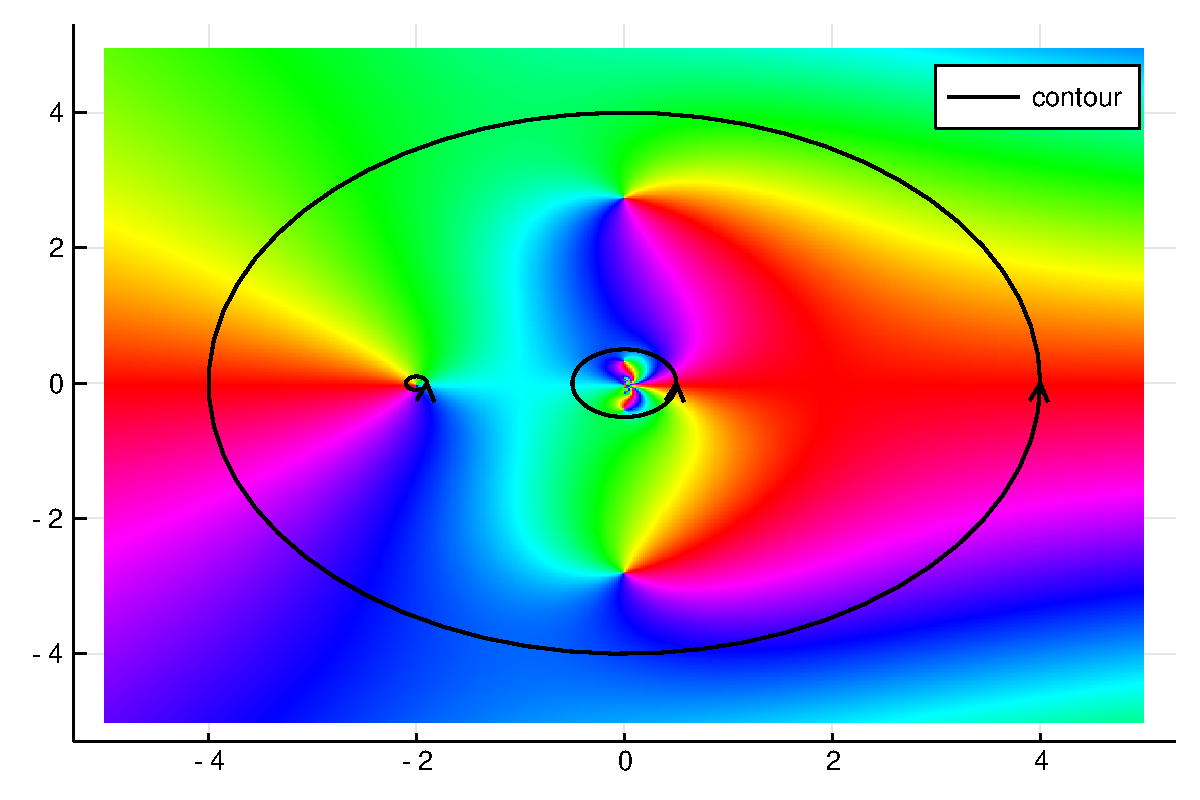
\includegraphics[width=\linewidth]{figures/Lecture11_1_1.pdf}

Cauchy's integral formula is still valid:


\begin{lstlisting}
(*@\HLJLn{\ensuremath{\zeta}}@*) (*@\HLJLoB{=}@*) (*@\HLJLnf{Fun}@*)(*@\HLJLp{(}@*)(*@\HLJLn{\ensuremath{\Gamma}}@*)(*@\HLJLp{)}@*)
(*@\HLJLn{z}@*) (*@\HLJLoB{=}@*) (*@\HLJLnfB{2.0}@*)(*@\HLJLoB{+}@*)(*@\HLJLnfB{1.0}@*)(*@\HLJLn{im}@*)
(*@\HLJLnf{sum}@*)(*@\HLJLp{(}@*)(*@\HLJLn{f}@*)(*@\HLJLoB{.}@*)(*@\HLJLp{(}@*)(*@\HLJLn{\ensuremath{\zeta}}@*)(*@\HLJLp{)}@*)(*@\HLJLoB{/}@*)(*@\HLJLp{(}@*)(*@\HLJLn{\ensuremath{\zeta}}@*) (*@\HLJLoB{-}@*) (*@\HLJLn{z}@*)(*@\HLJLp{))}@*)(*@\HLJLoB{/}@*)(*@\HLJLp{(}@*)(*@\HLJLni{2}@*)(*@\HLJLn{\ensuremath{\pi}}@*)(*@\HLJLoB{*}@*)(*@\HLJLn{im}@*)(*@\HLJLp{),}@*) (*@\HLJLnf{f}@*)(*@\HLJLp{(}@*)(*@\HLJLn{z}@*)(*@\HLJLp{)}@*)
\end{lstlisting}

\begin{lstlisting}
(0.8671607060038513 + 0.10261889457156066im, 0.8671607060038514 + 0.1026188
9457156062im)
\end{lstlisting}


Now we specialise to the case where we have a rational function 

\[
r(z) = {p(z) \over q(z)}
\]
where $p,q$ are both polynomials. This is analytic everywhere apart from the roots  of $q$, which we enumerate $\lambda_1,\ldots,\lambda_g$.   If we integrate over negatively oriented circles  around each root:


\begin{lstlisting}
(*@\HLJLn{n}@*) (*@\HLJLoB{=}@*) (*@\HLJLni{7}@*)
(*@\HLJLn{m}@*) (*@\HLJLoB{=}@*) (*@\HLJLni{5}@*)
(*@\HLJLn{p}@*) (*@\HLJLoB{=}@*) (*@\HLJLnf{Fun}@*)(*@\HLJLp{(}@*)(*@\HLJLnf{Taylor}@*)(*@\HLJLp{(),}@*) (*@\HLJLnf{randn}@*)(*@\HLJLp{(}@*)(*@\HLJLn{n}@*)(*@\HLJLp{))}@*)
(*@\HLJLn{q}@*) (*@\HLJLoB{=}@*) (*@\HLJLnf{Fun}@*)(*@\HLJLp{(}@*)(*@\HLJLnf{Taylor}@*)(*@\HLJLp{(),}@*) (*@\HLJLnf{randn}@*)(*@\HLJLp{(}@*)(*@\HLJLn{m}@*)(*@\HLJLp{))}@*)
(*@\HLJLn{\ensuremath{\lambda}}@*) (*@\HLJLoB{=}@*) (*@\HLJLnf{complexroots}@*)(*@\HLJLp{(}@*)(*@\HLJLn{q}@*)(*@\HLJLp{)}@*)

(*@\HLJLn{\ensuremath{\Gamma}}@*) (*@\HLJLoB{=}@*) (*@\HLJLnf{Circle}@*)(*@\HLJLp{(}@*)(*@\HLJLnfB{0.0}@*)(*@\HLJLp{,}@*) (*@\HLJLnfB{5.0}@*)(*@\HLJLp{)}@*)
(*@\HLJLk{for}@*) (*@\HLJLn{\ensuremath{\lambda}}@*) (*@\HLJLkp{in}@*) (*@\HLJLn{\ensuremath{\lambda}}@*)
    (*@\HLJLkd{global}@*) (*@\HLJLn{\ensuremath{\Gamma}}@*)
    (*@\HLJLn{\ensuremath{\Gamma}}@*) (*@\HLJLoB{=}@*) (*@\HLJLn{\ensuremath{\Gamma}}@*) (*@\HLJLoB{\ensuremath{\cup}}@*) (*@\HLJLnf{Circle}@*)(*@\HLJLp{(}@*)(*@\HLJLn{\ensuremath{\lambda}}@*)(*@\HLJLp{,}@*) (*@\HLJLnfB{0.1}@*)(*@\HLJLp{,}@*) (*@\HLJLkc{false}@*)(*@\HLJLp{)}@*)
(*@\HLJLk{end}@*)
(*@\HLJLn{r}@*) (*@\HLJLoB{=}@*) (*@\HLJLn{z}@*) (*@\HLJLoB{->}@*) (*@\HLJLnf{extrapolate}@*)(*@\HLJLp{(}@*)(*@\HLJLn{p}@*)(*@\HLJLp{,}@*)(*@\HLJLn{z}@*)(*@\HLJLp{)}@*)(*@\HLJLoB{/}@*)(*@\HLJLnf{extrapolate}@*)(*@\HLJLp{(}@*)(*@\HLJLn{q}@*)(*@\HLJLp{,}@*)(*@\HLJLn{z}@*)(*@\HLJLp{)}@*)

(*@\HLJLnf{phaseplot}@*)(*@\HLJLp{(}@*)(*@\HLJLoB{-}@*)(*@\HLJLnfB{5..5}@*)(*@\HLJLp{,}@*) (*@\HLJLoB{-}@*)(*@\HLJLnfB{5..5}@*)(*@\HLJLp{,}@*) (*@\HLJLn{r}@*)(*@\HLJLp{)}@*)
(*@\HLJLnf{plot!}@*)(*@\HLJLp{(}@*)(*@\HLJLn{\ensuremath{\Gamma}}@*)(*@\HLJLp{;}@*) (*@\HLJLn{color}@*)(*@\HLJLoB{=:}@*)(*@\HLJLn{black}@*)(*@\HLJLp{,}@*) (*@\HLJLn{label}@*)(*@\HLJLoB{=:}@*)(*@\HLJLn{contour}@*)(*@\HLJLp{)}@*)
\end{lstlisting}

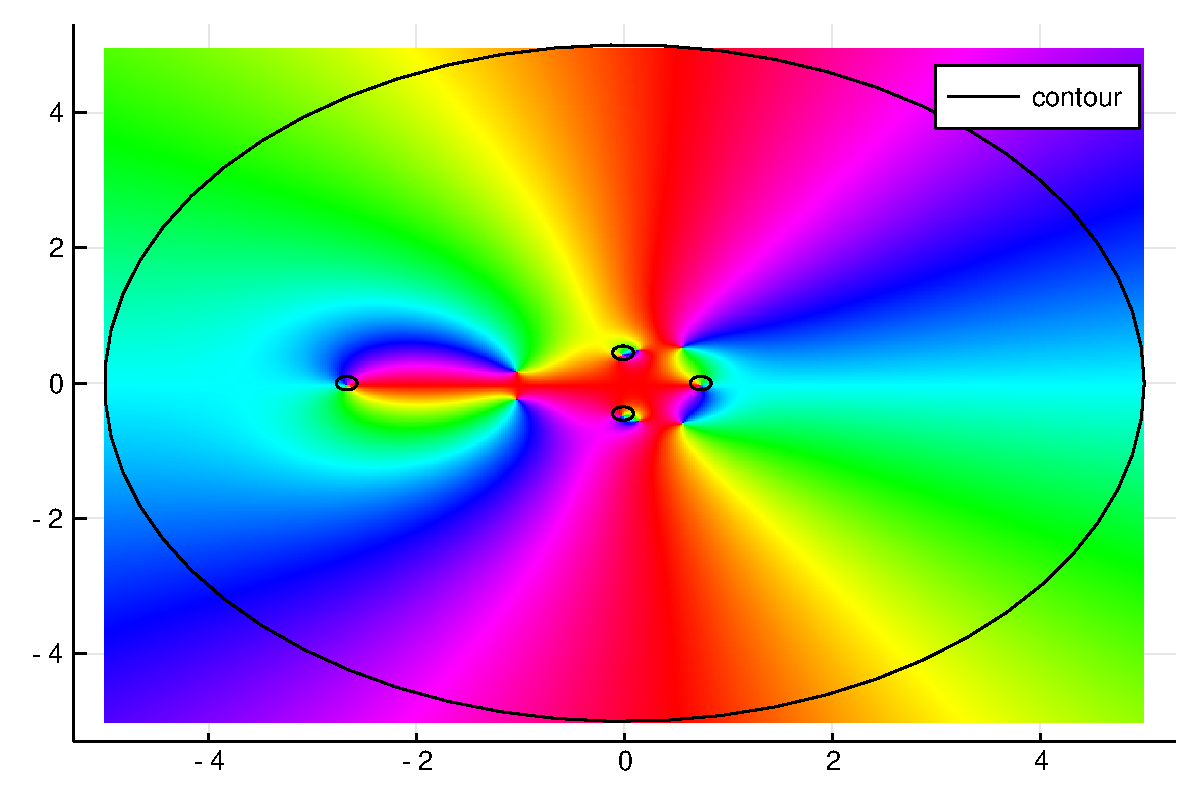
\includegraphics[width=\linewidth]{figures/Lecture11_3_1.pdf}

we recover the function:


\begin{lstlisting}
(*@\HLJLn{\ensuremath{\zeta}}@*) (*@\HLJLoB{=}@*) (*@\HLJLnf{Fun}@*)(*@\HLJLp{(}@*)(*@\HLJLn{\ensuremath{\Gamma}}@*)(*@\HLJLp{)}@*)
(*@\HLJLn{z}@*) (*@\HLJLoB{=}@*) (*@\HLJLnfB{2.0}@*)(*@\HLJLoB{+}@*)(*@\HLJLnfB{2.0}@*)(*@\HLJLn{im}@*)
(*@\HLJLnf{sum}@*)(*@\HLJLp{(}@*)(*@\HLJLn{r}@*)(*@\HLJLoB{.}@*)(*@\HLJLp{(}@*)(*@\HLJLn{\ensuremath{\zeta}}@*)(*@\HLJLp{)}@*)(*@\HLJLoB{/}@*)(*@\HLJLp{(}@*)(*@\HLJLn{\ensuremath{\zeta}}@*) (*@\HLJLoB{-}@*) (*@\HLJLn{z}@*)(*@\HLJLp{))}@*)(*@\HLJLoB{/}@*)(*@\HLJLp{(}@*)(*@\HLJLni{2}@*)(*@\HLJLn{\ensuremath{\pi}}@*)(*@\HLJLoB{*}@*)(*@\HLJLn{im}@*)(*@\HLJLp{)}@*) (*@\HLJLp{,}@*) (*@\HLJLnf{r}@*)(*@\HLJLp{(}@*)(*@\HLJLn{z}@*)(*@\HLJLp{)}@*)
\end{lstlisting}

\begin{lstlisting}
(4.372717213418816 - 46.349833892497706im, 4.372717213418801 - 46.349833892
497685im)
\end{lstlisting}


But now we can use the residue theorem to simplify the integrals! 

Near the $j$th root we have the Laurent series

\[
r(z) = r_{-N_j}^j (z-\lambda_j)^{-N_j}  + \cdots + r_{-1}^j (z-\lambda_j)^{-1} + r_0 + r_1 (z-\lambda_j) + \cdots
\]
where $N_j$ is the order of the zero of $q(z)$ at $\lambda_j$.

Then it follows that

\[
{1 \over 2 \pi \I} \oint_{\gamma_j} {r(\zeta) \over z - \zeta} \D\zeta = 
r_{-N_j}^j (z-\lambda_j)^{-N}  + \cdots + r_{-1}^j (z-\lambda_j)^{-1}
\]
for $z$ outside the contour $\gamma_j$.

Similarly, for the contour around infinity $\gamma_\infty$, if we have the Laurent series

\[
r(z) = \cdots + r_{-1}^\infty z^{-1} + r_0^\infty  + r_1^\infty z + \dots + r_{N_0}^\infty z^{N_0}
\]
where $N_\infty$ is the degree of $p(z)$ divided by the degree of $q(z)$.  Then we have

\[
{1 \over 2 \pi \I} \oint_{\gamma_\infty} {r(\zeta) \over z - \zeta} \D\zeta = 
r_0^\infty + r_1^\infty z + \cdots +  r_{N_0}^\infty z^{N_0}.
\]
Thus we have the expansion summing over the behaviour near each singularity that holds for all $z$:

\[
r(z) = \sum_{k=0}^{N_\infty} r_k^\infty z^k  +  \sum_{j=1}^d \sum_{k = -N_j}^{-1} r_k^j (z - \lambda_j)^k
\]
\emph{Example} When we only have simple poles and no polynomial growth at $\infty$, this has a simple form in terms of residues:

\[
r(z) = r(\infty)  +  \sum_{j=1}^d    (z - \lambda_j)^{-1} \underset{z = \lambda_j}{\rm Res}\, r(z)
\]
Here we demonstrate it on a random polynomial:


\begin{lstlisting}
(*@\HLJLn{n}@*) (*@\HLJLoB{=}@*) (*@\HLJLni{5}@*)
(*@\HLJLn{m}@*) (*@\HLJLoB{=}@*) (*@\HLJLni{5}@*)
(*@\HLJLn{p}@*) (*@\HLJLoB{=}@*) (*@\HLJLnf{Fun}@*)(*@\HLJLp{(}@*)(*@\HLJLnf{Taylor}@*)(*@\HLJLp{(),}@*) (*@\HLJLnf{randn}@*)(*@\HLJLp{(}@*)(*@\HLJLn{n}@*)(*@\HLJLp{))}@*)
(*@\HLJLn{q}@*) (*@\HLJLoB{=}@*) (*@\HLJLnf{Fun}@*)(*@\HLJLp{(}@*)(*@\HLJLnf{Taylor}@*)(*@\HLJLp{(),}@*) (*@\HLJLnf{randn}@*)(*@\HLJLp{(}@*)(*@\HLJLn{m}@*)(*@\HLJLp{))}@*)
(*@\HLJLn{\ensuremath{\lambda}}@*) (*@\HLJLoB{=}@*) (*@\HLJLnf{complexroots}@*)(*@\HLJLp{(}@*)(*@\HLJLn{q}@*)(*@\HLJLp{)}@*)

(*@\HLJLn{r}@*) (*@\HLJLoB{=}@*) (*@\HLJLn{z}@*) (*@\HLJLoB{->}@*) (*@\HLJLnf{extrapolate}@*)(*@\HLJLp{(}@*)(*@\HLJLn{p}@*)(*@\HLJLp{,}@*)(*@\HLJLn{z}@*)(*@\HLJLp{)}@*)(*@\HLJLoB{/}@*)(*@\HLJLnf{extrapolate}@*)(*@\HLJLp{(}@*)(*@\HLJLn{q}@*)(*@\HLJLp{,}@*)(*@\HLJLn{z}@*)(*@\HLJLp{)}@*)

(*@\HLJLnf{phaseplot}@*)(*@\HLJLp{(}@*)(*@\HLJLoB{-}@*)(*@\HLJLnfB{7..7}@*)(*@\HLJLp{,}@*) (*@\HLJLoB{-}@*)(*@\HLJLnfB{7..7}@*)(*@\HLJLp{,}@*) (*@\HLJLn{r}@*)(*@\HLJLp{)}@*)
\end{lstlisting}

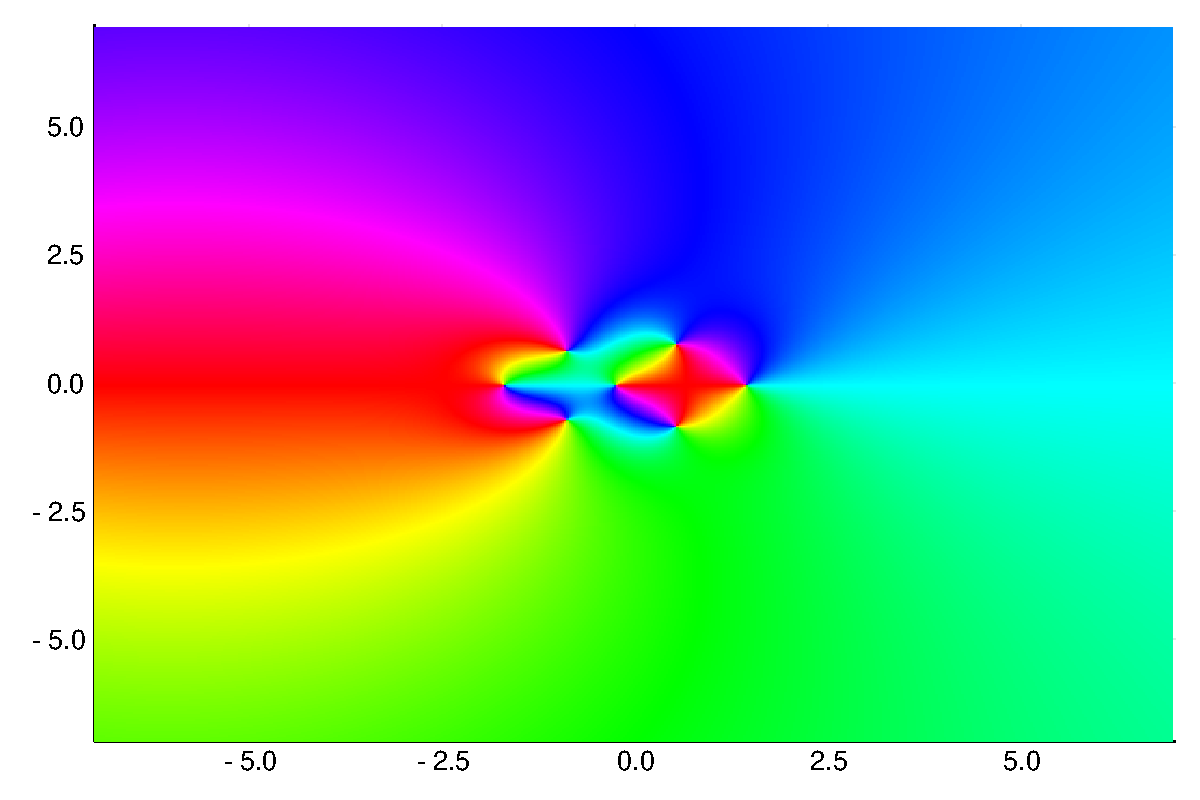
\includegraphics[width=\linewidth]{figures/Lecture11_5_1.pdf}

This constructs \texttt{r\_2} as the partial fraction expansion of \texttt{r}:


\begin{lstlisting}
(*@\HLJLn{res}@*) (*@\HLJLoB{=}@*) (*@\HLJLn{extrapolate}@*)(*@\HLJLoB{.}@*)(*@\HLJLp{(}@*)(*@\HLJLn{p}@*)(*@\HLJLp{,}@*)(*@\HLJLn{\ensuremath{\lambda}}@*)(*@\HLJLp{)}@*)(*@\HLJLoB{./}@*)(*@\HLJLn{extrapolate}@*)(*@\HLJLoB{.}@*)(*@\HLJLp{(}@*)(*@\HLJLn{q}@*)(*@\HLJLoB{{\textquotesingle}}@*)(*@\HLJLp{,}@*)(*@\HLJLn{\ensuremath{\lambda}}@*)(*@\HLJLp{)}@*)
(*@\HLJLn{r\ensuremath{\infty}}@*) (*@\HLJLoB{=}@*) (*@\HLJLn{p}@*)(*@\HLJLoB{.}@*)(*@\HLJLn{coefficients}@*)(*@\HLJLp{[}@*)(*@\HLJLn{n}@*)(*@\HLJLp{]}@*)(*@\HLJLoB{/}@*)(*@\HLJLn{q}@*)(*@\HLJLoB{.}@*)(*@\HLJLn{coefficients}@*)(*@\HLJLp{[}@*)(*@\HLJLn{m}@*)(*@\HLJLp{]}@*)

(*@\HLJLn{r{\_}2}@*) (*@\HLJLoB{=}@*) (*@\HLJLn{z}@*) (*@\HLJLoB{->}@*) (*@\HLJLn{r\ensuremath{\infty}}@*) (*@\HLJLoB{+}@*) (*@\HLJLnf{sum}@*)(*@\HLJLp{(}@*)(*@\HLJLn{res}@*)(*@\HLJLoB{.*}@*)(*@\HLJLp{(}@*)(*@\HLJLn{z}@*) (*@\HLJLoB{.-}@*) (*@\HLJLn{\ensuremath{\lambda}}@*)(*@\HLJLp{)}@*)(*@\HLJLoB{.{\textasciicircum}}@*)(*@\HLJLp{(}@*)(*@\HLJLoB{-}@*)(*@\HLJLni{1}@*)(*@\HLJLp{))}@*)

(*@\HLJLn{z}@*) (*@\HLJLoB{=}@*) (*@\HLJLnfB{0.1}@*)(*@\HLJLoB{+}@*)(*@\HLJLnfB{0.2}@*)(*@\HLJLn{im}@*)
(*@\HLJLnf{r}@*)(*@\HLJLp{(}@*)(*@\HLJLn{z}@*)(*@\HLJLp{)}@*) (*@\HLJLoB{-}@*) (*@\HLJLnf{r{\_}2}@*)(*@\HLJLp{(}@*)(*@\HLJLn{z}@*)(*@\HLJLp{)}@*) (*@\HLJLcs{{\#}}@*) (*@\HLJLcs{we}@*) (*@\HLJLcs{match}@*) (*@\HLJLcs{to}@*) (*@\HLJLcs{high}@*) (*@\HLJLcs{accuracy}@*)
\end{lstlisting}

\begin{lstlisting}
0.0 + 8.153200337090993e-16im
\end{lstlisting}


\subsection{Recovering analytic functions}
We now consider the above approach for 2 examples with branch cuts.

\textbf{Example 1}

Consider $\phi(z) = \log(z-1) - \log(z+1)$. For $x < -1$ the branch cuts cancel  and we have

\[
\phi_+(x) = \lim \phi(x + \I \epsilon) = \log_+(x-1) - \log_+(x+1) = 
\log|x-1| + \I \pi - \log|x+1| - \I \pi = \log(1-x) - \log(-1-x).
\]
Similarly

\[
\phi_-(x) =  \log(1-x) - \log(-1-x) = \phi_+(x)
\]
i.e., we are continuous on the branch cut (with $\phi(x) := \phi_+(x)$) and therefore analytic. Thus $\phi(z)$ is analytic off $[-1,1]$ which can be seen clearly from a phase portrait. Using the corollary above we can recover $f$ from integrating over two contours: $\gamma_\infty$ surrounding $\infty$  and $\gamma_0$ surrounding the branch cut, with $z$ in-between:


\begin{lstlisting}
(*@\HLJLn{\ensuremath{\varphi}}@*) (*@\HLJLoB{=}@*) (*@\HLJLn{z}@*) (*@\HLJLoB{->}@*) (*@\HLJLnf{log}@*)(*@\HLJLp{(}@*)(*@\HLJLn{z}@*)(*@\HLJLoB{-}@*)(*@\HLJLni{1}@*)(*@\HLJLp{)}@*) (*@\HLJLoB{-}@*) (*@\HLJLnf{log}@*)(*@\HLJLp{(}@*)(*@\HLJLn{z}@*)(*@\HLJLoB{+}@*)(*@\HLJLni{1}@*)(*@\HLJLp{)}@*)
(*@\HLJLnf{phaseplot}@*)(*@\HLJLp{(}@*)(*@\HLJLoB{-}@*)(*@\HLJLnfB{3..3}@*)(*@\HLJLp{,}@*) (*@\HLJLoB{-}@*)(*@\HLJLnfB{3..3}@*)(*@\HLJLp{,}@*) (*@\HLJLn{\ensuremath{\varphi}}@*)(*@\HLJLp{)}@*)
(*@\HLJLn{\ensuremath{\theta}}@*) (*@\HLJLoB{=}@*) (*@\HLJLnf{range}@*)(*@\HLJLp{(}@*)(*@\HLJLni{0}@*)(*@\HLJLp{,}@*)(*@\HLJLni{2}@*)(*@\HLJLn{\ensuremath{\pi}}@*)(*@\HLJLp{;}@*) (*@\HLJLn{length}@*)(*@\HLJLoB{=}@*)(*@\HLJLni{200}@*)(*@\HLJLp{)}@*)
(*@\HLJLnf{plot!}@*)(*@\HLJLp{(}@*)(*@\HLJLnfB{2.5}@*)(*@\HLJLn{cos}@*)(*@\HLJLoB{.}@*)(*@\HLJLp{(}@*)(*@\HLJLn{\ensuremath{\theta}}@*)(*@\HLJLp{),}@*) (*@\HLJLnfB{2.5}@*)(*@\HLJLn{sin}@*)(*@\HLJLoB{.}@*)(*@\HLJLp{(}@*)(*@\HLJLn{\ensuremath{\theta}}@*)(*@\HLJLp{);}@*) (*@\HLJLn{color}@*)(*@\HLJLoB{=:}@*)(*@\HLJLn{black}@*)(*@\HLJLp{,}@*) (*@\HLJLn{label}@*)(*@\HLJLoB{=}@*)(*@\HLJLs{"{}}@*)(*@\HLJLse{{\textbackslash}{\textbackslash}}@*)(*@\HLJLs{gamma{\_}inf"{}}@*)(*@\HLJLp{,}@*) (*@\HLJLn{arrow}@*)(*@\HLJLoB{=}@*)(*@\HLJLkc{true}@*)(*@\HLJLp{)}@*)
(*@\HLJLnf{plot!}@*)(*@\HLJLp{(}@*)(*@\HLJLnfB{1.2}@*)(*@\HLJLn{cos}@*)(*@\HLJLoB{.}@*)(*@\HLJLp{(}@*)(*@\HLJLn{\ensuremath{\theta}}@*)(*@\HLJLp{),}@*) (*@\HLJLnfB{0.2}@*)(*@\HLJLn{sin}@*)(*@\HLJLoB{.}@*)(*@\HLJLp{(}@*)(*@\HLJLoB{-}@*)(*@\HLJLn{\ensuremath{\theta}}@*)(*@\HLJLp{);}@*) (*@\HLJLn{color}@*)(*@\HLJLoB{=:}@*)(*@\HLJLn{blue}@*)(*@\HLJLp{,}@*) (*@\HLJLn{label}@*)(*@\HLJLoB{=}@*)(*@\HLJLs{"{}}@*)(*@\HLJLse{{\textbackslash}{\textbackslash}}@*)(*@\HLJLs{gamma{\_}0"{}}@*)(*@\HLJLp{,}@*) (*@\HLJLn{arrow}@*)(*@\HLJLoB{=}@*)(*@\HLJLkc{true}@*)(*@\HLJLp{)}@*)
(*@\HLJLnf{scatter!}@*)(*@\HLJLp{([}@*)(*@\HLJLnfB{0.1}@*)(*@\HLJLp{],[}@*)(*@\HLJLnfB{0.5}@*)(*@\HLJLp{];}@*) (*@\HLJLn{label}@*)(*@\HLJLoB{=}@*)(*@\HLJLs{"{}z"{}}@*)(*@\HLJLp{)}@*)
\end{lstlisting}

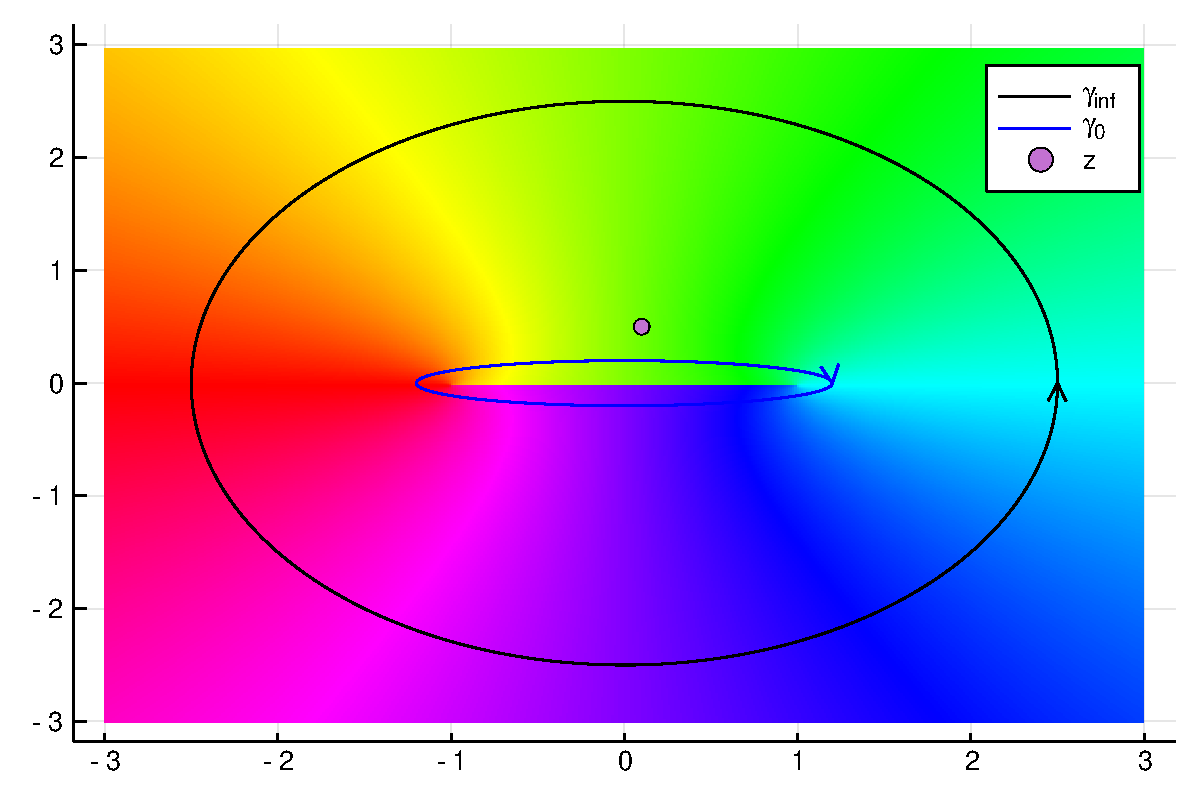
\includegraphics[width=\linewidth]{figures/Lecture11_7_1.pdf}

That is, we have

\[
\phi(z) = {1 \over 2 \pi \I} \br[\oint_{\gamma_0} + \oint_{\gamma_\infty}] {\phi(\zeta) \over \zeta -z} \D \zeta
\]
Note that $\phi(z)$ is analytic in a neighbourhood of $\infty$ and has weaker-than-pole growth: it can only grow at worse like $\log z$. Thus it must be analytic at $\infty$. To determine the  constant we use a simple Taylor series argument, evaluating on the real axis to simplify rules of  logarithms: as $x \rightarrow \infty$ we have

\[
\phi(x) = \log(x-1) - \log(x+1) = \log x + \log(1-1/x) - \log x - \log(1 +1/x) \rightarrow 0,
\]
that is $\phi(\infty) = 0$, and in fact $\phi(z) = O(z^{-1})$ as $\phi(z^{-1})$ is analytic at zero and therefore has a converging Taylor series.  It follows from Cauchy's theorem (exterior) that

\[
\oint_{\gamma_\infty} {\phi(\zeta) \over \zeta -z} \D \zeta = 0
\]
as the integrand decays like $O(\zeta^{-2})$. 

We are left with the integral on $\gamma_0$. We can think of it as a rectangular contour with contours  $[-1-\epsilon-\I \epsilon, -1 -\epsilon+\I \epsilon,1 +\epsilon+\I\epsilon,1+\epsilon-\I \epsilon]$. Letting $\epsilon \rightarrow 0$, on the contour above $\phi(z)$ tends to 

\[
\lim_{\epsilon \rightarrow 0} \phi(x + \I \epsilon) = \phi_+(x)
\]
and similar to the contour below. Since $\phi$ only has logarithmic singularities this limit can be done safely. Thus we end up with the expression

\[
\phi(z) = {1 \over 2 \pi \I} \oint_{\gamma_0} {\phi(\zeta) \over \zeta -z} \D \zeta = 
        {1 \over 2 \pi \I} \int_{-1}^1 {\phi_+(x) - \phi_-(x) \over x - z} \D x = \int_{-1}^1 {1 \over x -z} \D x.
\]
\textbf{Example 2}

We repeat the above procedure with $\phi(z) = \sqrt{z-1} \sqrt{z+1}$. Again this is analytic off $[-1,1]$ and we can express it as integrals over $\gamma_0$ and $\gamma_\infty$. Now it grows like $z$ at $\infty$,

\[
\phi(z) = z + O(z^{-1}),
\]
hence we have (as above)

\[
{1 \over 2 \pi \I} \oint_{\gamma_\infty} {\phi(\zeta) \over \zeta - z} \D \zeta = z.
\]
The integral over the contour $\gamma_0$ can be collapsed. On the jump $-1 < x < 1$ we have 

\[
\phi_+(x) = \sqrt{x-1}_+ \sqrt{x+1} = \I \sqrt{|x-1|} \sqrt{x+1} = \I \sqrt{1-x} \sqrt{x+1} = \I \sqrt{1-x^2}
\]
while $\phi_-(x) = - \phi_+(x) = - \I \sqrt{1-x^2}$. We thus have


\begin{align*}
\phi(z) &= z + {1 \over 2 \pi \I} \oint_{\gamma_0} {\phi(\zeta) \over \zeta -z} \D \zeta = 
        z + {1 \over 2 \pi \I} \int_{-1}^1 {\phi_+(x) - \phi_-(x) \over x - z} \D x \\
        &= 
        z + {1 \over \pi} \int_{-1}^1 {\sqrt{1-x^2} \over x -z} \D x.
\end{align*}


\end{document}
